\section{Experimental Evaluation}\label{results}






% No attack was able to leak, but number of false positive increased. 



% Accuracy on 3-fold cross validation improved by 7\%


% We take an attack sample first and project it back to the latent space $z$.
% We use the generator $G$ to generate a similar example to $x$, called ${x^{\star}}$ by $G(z)$. Then we use the classifier $C$ to classify the example $C(x^{\star})$, which generally already tends to misclassify way less than running the classification directly on $x$. 

\textcolor{red}{DMT: Okay, I need help understanding this graph.  I'm not sure how that first sentence
comes out of this graph.  Is the training set the first N (?) training examples, and the synthetic 
examples the next 400-N?  And don't you generated many more synthetic examples than that?
}

 Performance of our new classifier does drop on the training set, but accuracy improves on test set including adversarial attacks. Figure~\ref{fig:accuracy} shows \scheme achieves significant improvement in classification accuracy as the number of training examples increases, especially synthetic examples produced by adversarial perSpectron. The dotted line depicts classification performance for classic data augmentation using program synthesizers. The performance improves as the quantity of new (augmented) training examples increases; however, the improvement plateaus around the accuracy of 78\%, (78.14717909)
 beyond which additional examples fail to yield improvement.
 
\begin{figure}[ht!] 
\centering
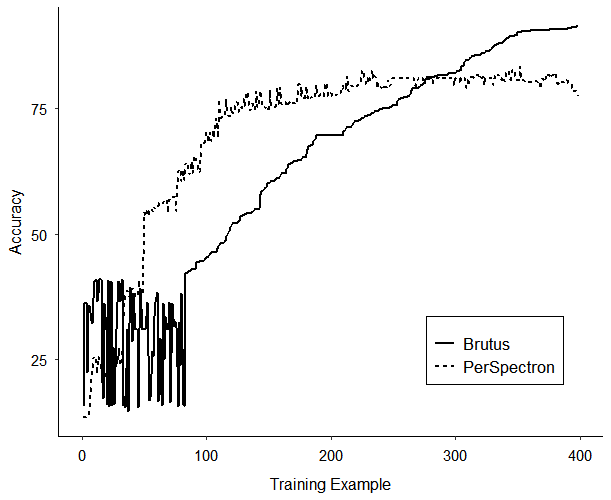
\includegraphics[width=0.49\textwidth]{PerSpectron-Micro2020-camera-R/img/adverse88.png}
\vspace*{-4mm}
\caption{Comparing detection accuracy shows 
  \scheme{} 
}
\label{fig:accuracy}
\end{figure}

The solid line shows the additional increase in accuracy achieved by augmenting the adversarial examples using GAN-trained DNN against adversarial PerSpectron. Starting from the point beyond which additional classically augmented examples stopped improving accuracy, we added synthetic data generated by our trained DNN/adversarial perSpectron GAN. The classification performance improved to over 90\% (91.14454905), demonstrating the usefulness of \scheme. 

\textcolor{red}{DMT: So if you put the original perspectron on this graph (which seems appropriate), would
it be a straight line or also a sloped asymptote?}

% Figure shows the loss value of generator vs training epoch for a range of features. Using a few high level features would result in discriminator losing the game to the generator faster. we define the new metric {\em Nash Equilibrium Speed} to be the loss of generative model over 1000 epochs. that is proportional to the vulnerability to adversarial machine learning attack and  inversely proportional  to the resiliency of a model to adversarial machine learning attacks. 

% People have noted that adding labels to the data—that is, to break it up into categories, almost always improves the performance of GANs.

% Generated data, showing high features in .. which is high in all the variations. 


% Table shows the attack success rate under attacks, inclduing {\scheme} and other synthetization base technique and original PerSpectron. We can see that {\scheme} outperforms others. 
% Again we have to emphesize that unlike other perturbation techniques, {\scheme} cannot limit the size of perturbation by nature so it is not surprizing higher 